\chapter{Aspectos generales}
\doublespacing
%En esta sección se va desde aspectos generales a  aspectos específicos (como un embudo). No se olvide que es la primera parte que tiene contacto con el lector y que hará que este se interese en el tema a investigar.
%El objetivo de esta sección es llevar al lector hacie el tema que se va a tratar en forma específica y dejar la puerta abierta a otras investigaciones.
\section{Ámbito geográfico}
El desarrollo de la tesis tendra como área de estudio el glaciar Quelccaya, el cual se encuentra sobre una amplia meseta al sureste del Perú, en la Cordillera Vilcanota, entre los departamentos de Cusco y Puno. Considerada la segunda capa de hielo tropical mas grande del mundo \parencite{malone2022evolution}, \parencite{taylor2022multi}. La elevación media del margen de hielo es de 5300 m.s.n.m. y la elevación aproximada de la cumbre es de 5680 m.s.n.m. \parencite{yarleque2018projections}


\begin{figure}[h!]
	\centering
	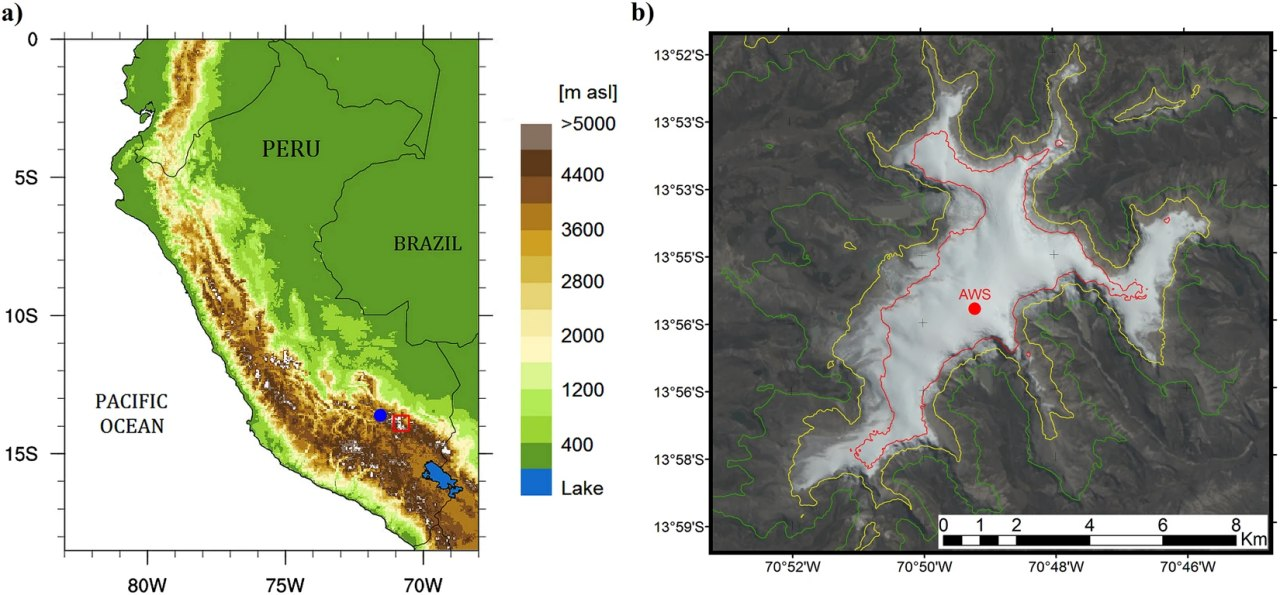
\includegraphics[width=0.98\linewidth]{graficos/area}
	\caption[Ubicación del manto glaciar Quelccaya]{Ubicación del manto glaciar Quelccaya, (a) Topografía de los Andes, ubicación del glaciar Quelccaya (cuadrado rojo). (b) Imagen RGB LANDSAT 8 del glaciar Quelccaya obtenida el 2 de agosto de 2017. La ubicación AWS se muestra con un punto rojo. Los contornos de color representan las isolíneas 5100 (verde), 5300 (amarillo) y 5500~m~s.n.m. (rojas)
	
	Fuente: \parencite{yarleque2018projections}}
	\label{fig:area}
\end{figure}

\section{Descripción de la realidad problemática}

El retroceso glaciar en los Andes del Perú es un fenómeno preocupante que ha estado ocurriendo en las últimas décadas y que tiene fuertes vínculos con la contaminación global y el cambio climático. Los glaciares en la región andina han experimentado una disminución significativa en su tamaño y volumen, lo que se conoce como retroceso glaciar. El aumento de la temperatura a nivel global llega a tener impactos directos en los glaciares, pues contribuye al derretimiento acelerado y al retroceso de las masas de hielo en las altas montañas \parencite{drenkhan2018current}.

El Perú, hogar de una porción significativa de la biodiversidad global, concentra el 68{\%} de los glaciares tropicales del mundo según \parencite{inaigem2023}. Sin embargo, debido al acelerado retroceso de la superficie de los glaciares, se estima que para el 2030 disminuya en un 6{\%} la disponibilidad hídrica en la vertiente del pacífico, esto llega a generar una gran problemática para el consumo humano, sistemas de riego y generación de energía eléctrica \parencite{ruiz2023deglaciacion}.  Pues estos glaciares en el Perú llegan a ser grandes reservas de agua dulce, sin embargo, recientes estudios de \parencite{aliaga2018retroceso} indican que en los últimos 35 años se ha perdido cerca del 22{\%} de la superficie glaciar, esto fue evidenciado en una comparativa que se realizó entre los años 1970 teniendo una superficie glaciar equivalente a 1958 km\textsuperscript{2}, 2006 teniendo una superficie glaciar equivalente a 1370 km\textsuperscript{2} y registros actualizados al 2010 equivalente a 1230 km\textsuperscript{2} de superficie .

Además, La Cordillera del Vilcanota provee de agua al valle del río Vilcanota, en este valle se concentra el 75{\%} de la población del Departamento del Cusco, 82{\%} de terrenos de cultivos lo cual llega a constituir parte importante de la economía de los pobladores. En este valle se encuentran ciudades como Tinta, Sicuani, Combapata, Urcos, Pisaq, Calca, Urubamba, Ollantaytambo, Machupicchu, Quillabamba, etc.  \parencite{porcel2015iniciacion}. La Central Hidroeléctrica de Machupicchu,  fuente de energía que abastece a todo el departamento de Cusco, está ubicado en el curso medio del rio Vilcanota, el río proporciona 131 m$^3/$s de agua promedio anual para la Central Hidroeléctrica \parencite{cabrera2019curvas}


Cabe recalcar que la Cordillera Vilcanota en el sur de Perú, es considerada como la segunda cadena glaciar con mayor presencia de nieve en Perú y sus nevados Cayangate, Tacusiri, Surimani, Qolpacunca, Chimboya, Chumpi, Ambroca, y el glaciar de Quelccaya, son de gran importancia a nivel hídrico en la región, siendo actualmente el Quelcaya el segundo glaciar más extenso del mundo y plano en la zona tropical y es de gran interés científico, pues permite estimar el ritmo de desglaciación de estas montañas y analizar los cambios climáticos ocurridos en el trópico desde la última era glaciar \parencite{taylor2022multi}. Además, alberga uno de los lagos alpinos más grandes, Sibinacocha. Es en esta zona donde el Telmatobius marmoratus (rana de agua veteada), Rhinella spinulosa (sapo andino) y Pleurodema marmoratum (rana de cuatro ojos veteada) han ampliado su área de distribución para habitar en estanques recién formados que fueron creados a causa de la deglaciación en curso, según \parencite{seimon2017long} revela cambios dinámicos en el hábitat que es afectada por la deglaciación en curso, pues se genera la formación de nuevos estanques, cambios en la vegetación en el hábitat de los anfibios. Por lo tanto, mantener la humedad en la Cordillera Vilcanota es esencial para garantizar la supervivencia de estas especies, adaptándose al cambio climático continuo.

%%%%%%%%%%%%%%%%%%%%%%%%%%%%%%%%%%%%%%%%%%%%%%%%%%%%%%
El casquete de hielo de Quelccaya, ubicado en una meseta de gran altitud en los Andes peruanos, está sufriendo los efectos del cambio climático a pesar de las temperaturas frías en estas alturas. Entre 1988 y 2023, la extensión del glaciar se redujo de 58 km² a 40 km², según estimaciones de Christopher Shuman, glaciólogo de la Universidad de Maryland y colaborador de la NASA. Este retroceso ha sido documentado mediante imágenes satelitales Landsat, que también han revelado la aparición y desaparición de lagos glaciares durante este periodo. En particular, en noviembre de 2022, un desbordamiento violento de un lago glaciar causó una inundación, dejando una cicatriz visible en las imágenes de 2023 \parencite{nasa2024}.

Desde 1974, Lonnie Thompson y su equipo de la Universidad de Ohio han liderado investigaciones sobre el casquete de Quelccaya, documentando su retroceso con imágenes terrestres y satelitales. Además, el equipo ha perforado núcleos de hielo del glaciar, proporcionando un registro histórico de la temperatura y la composición atmosférica que se remonta a 1.800 años. Además estos glaciares tropicales ofrecen una valiosa oportunidad para comprender los cambios en la temperatura media global y el clima en áreas que representan más del 50 \% de la superficie del planeta, donde vive más del 50 \% de la población mundial. Sin embargo, se estima que el casquete de hielo de Quelccaya podría desaparecer antes de que termine el siglo XXI, dejando solo imágenes terrestres y satelitales como testimonio de su existencia \parencite{nasa2024}.



\begin{figure}[h]
	\centering
	\begin{minipage}{\textwidth} % Utilizamos un minipage para controlar la alineación
		%\raggedright % Asegura que la caption esté alineada a la izquierda
		\caption{ \raggedright \\
			 \textit{Incidencia de anemia por grupo etario y según residencia.}} % Alineado a la izquierda
		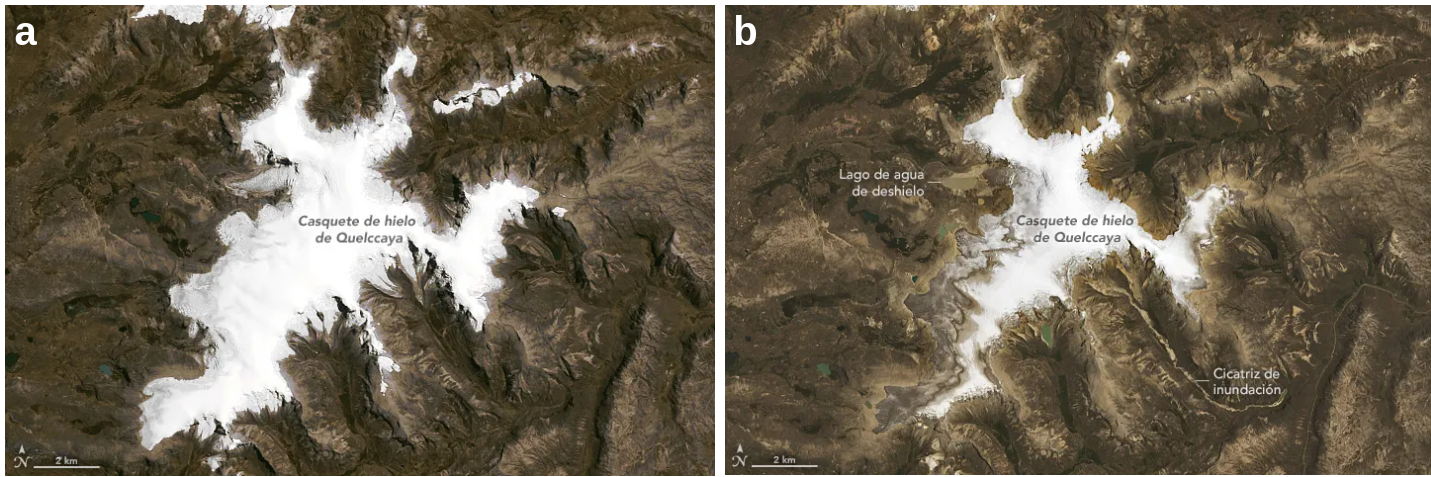
\includegraphics[width=13.5cm]{graficos/quelccaya_cambio} % Imagen centrada
		\caption*{\normalsize \textbf{Nota:} Retroceso superficial del Glaciar Quelccaya vista a través de una imagen satelital. 
			a) Imagen de 3 de septiembre de 1988, b) Imagen del 22 de octubre de 2023. \\
			\textbf{Fuente:} Elaboración propia.} % Nota alineada a la izquierda
	\end{minipage}
	\label{fig1}
\end{figure}


\begin{figure}[h]
	\centering
	
	\caption{ \raggedright \\
		\textit{Incidencia de anemia por grupo etario y según residencia.}} % Alineado a la izquierda
	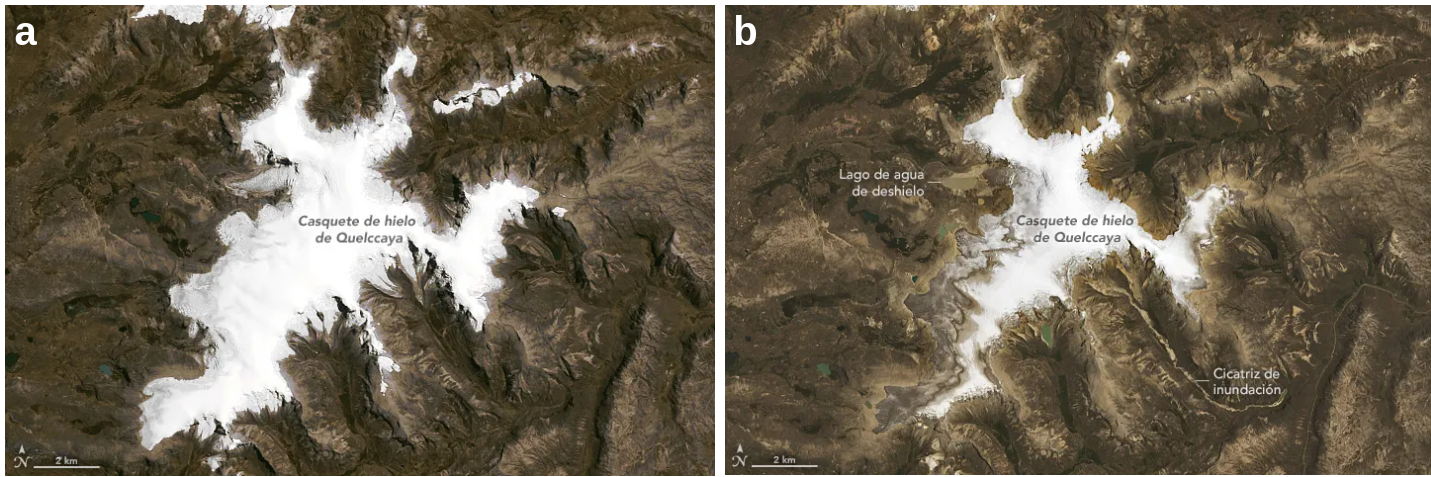
\includegraphics[width=13.5cm]{graficos/quelccaya_cambio} % Imagen centrada
	\caption*{\normalsize \textbf{Nota:} Retroceso superficial del Glaciar Quelccaya vista a través de una imagen satelital. 
		a) Imagen de 3 de septiembre de 1988, b) Imagen del 22 de octubre de 2023. \\
		\textbf{Fuente:} Elaboración propia.} % Nota alineada a la izquierda
	
	\label{fig:quelc}
\end{figure}


\begin{figure}[h!]
	\centering
	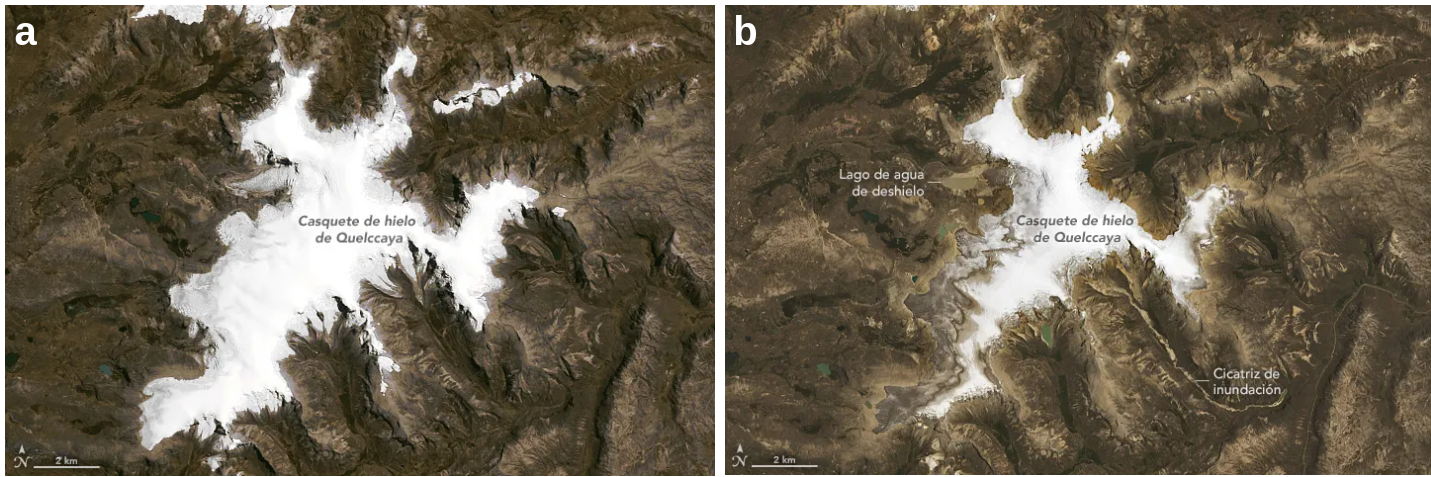
\includegraphics[width=0.7\linewidth]{graficos/quelccaya_cambio}
	\caption*{\normalsize \textbf{Nota:} Retroceso superficial del Glaciar Quelccaya vista a través de una imagen satelital. 
		a) Imagen de 3 de septiembre de 1988, b) Imagen del 22 de octubre de 2023. \\
		\textbf{Fuente:} Elaboración propia.} % Nota alineada a la izquierda
\end{figure}


\begin{figure}[h!]
	\centering
	\caption{ \raggedright \\
		\textit{Incidencia de anemia por grupo etario y según residencia.}} % Alineado a la izquierda
	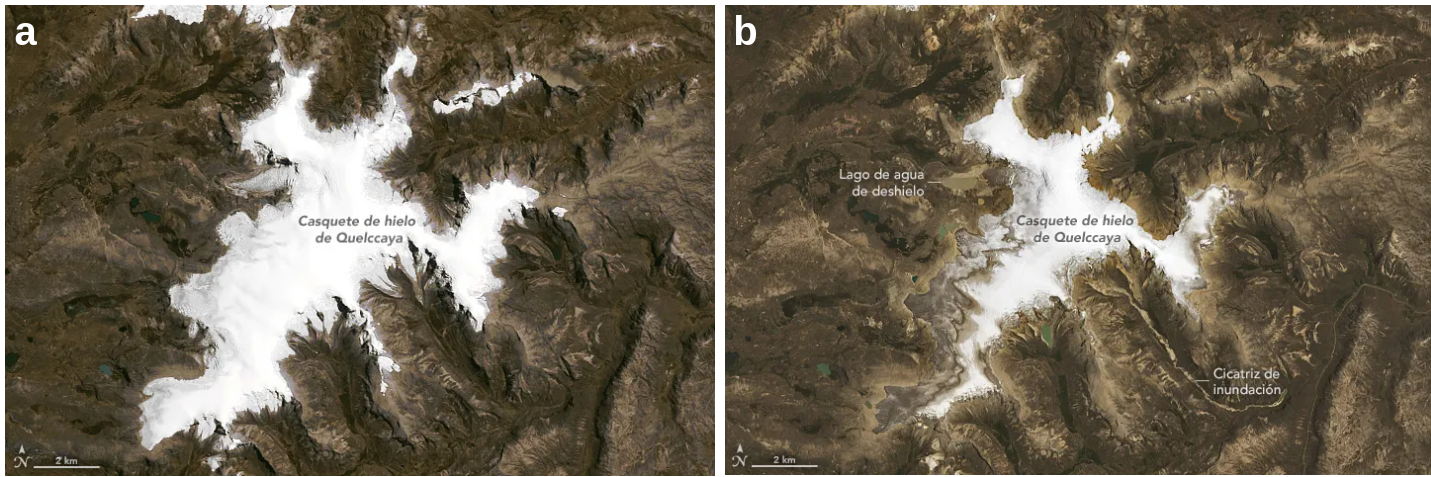
\includegraphics[width=0.7\linewidth]{graficos/quelccaya_cambio}
	\caption[Retroceso superficial del Glaciar Quelccaya vista a travéz de una imagen satelital.]{Retroceso superficial del Glaciar Quelccaya vista a travéz de una imagen satelital. a) Imagen de 3 de septiembre de 1988, b) Imagen del 22 de octubre de 2023.
		
		Fuente: \url{https://ciencia.nasa.gov/ciencias-terrestres/el-casquete-de-hielo-de-quelccaya-antes-y-ahora/}.}
	\label{fig:quelccaya_cambio}
\end{figure}


Según la revista \parencite{ojopublico2024}, a casi 5,000 metros de altitud, la comunidad de Phinaya, en los Andes peruanos, trabaja para proteger uno de los glaciares tropicales más importantes del mundo: el Quelccaya. El calentamiento global está acelerando el deshielo de este vasto glaciar, pero las comunidades quechuas han unido esfuerzos para mitigar los impactos de su retroceso. La revista indica que en 1982, el Quelccaya era el glaciar tropical más grande del mundo. Cuatro décadas después, su superficie ha disminuido un 46 \%, dejándolo en segundo lugar tras el Nevado Coropuna. Esta pérdida ha dejado a las 200 familias de Phinaya en una zona amenazada por la desertificación, enfrentando serios problemas de acceso al agua.

Una entrevista por parte de la revista realizada a Yolanda Quispe, guardaparques y comunera de Phinaya, expresa con emoción que proteger el glaciar es un honor, dado que representa un pilar fundamental para la vida en la región. En 2019, las comunidades de Phinaya y la Asociación de Vivienda Salma Sallani se unieron al Área de Conservación Regional (ACR) Ausangate, protegiendo unas 66,500 hectáreas de ecosistemas frágiles en la cordillera de Vilcanota.

Además el ACR busca conservar las áreas montañosas, que son fuente de agua y hábitat para diversas especies. Sin embargo, el deshielo del Quelccaya no solo afecta a la biodiversidad, sino también a las familias que dependen del pastoreo de alpacas, la principal actividad económica de la comunidad. Con el cambio climático secando los pastizales, la crianza de estos animales se ha vuelto insostenible, incrementando la migración hacia las ciudades cercanas \parencite{ojopublico2024}.

La migración es ahora impulsada por el deterioro de los recursos naturales, lo que ha provocado que muchos jóvenes abandonen la comunidad según estudios recientes de \parencite{costa2022migraccoes}. Esta pérdida de población no solo amenaza la continuidad de las actividades tradicionales, sino que también abre la puerta a la explotación minera, lo que podría generar más conflictos y degradación ambiental. Frente a esta situación, el ACR Ausangate busca promover el ecoturismo como una estrategia para atraer a los jóvenes de regreso a la comunidad, protegiendo a la vez los ecosistemas y la cultura local \parencite{ojopublico2024}.
%%%%%%%%%%%%%%%%%%%%%%%%%%%%%%%%%%%%%%%%%%%%%%%%%%%%%%%%%%


La función crucial de los glaciares como reservorios temporales de agua adquiere una relevancia especial en regiones tropicales, dada la presencia de dos estaciones bien definidas, una lluviosa y otra seca. A pesar de su papel fundamental, son escasas las investigaciones sobre el balance de masa en los glaciares de la Cordillera Vilcanota. \parencite{porcel2015iniciacion}

La conservación de las cuencas en la Cordillera del Vilcanota tiene gran importancia debido a que constituyen la fuente de suministro de agua para una extensa área en la región de Cusco. Además, son fundamentales para el desarrollo de la actividad turística, que atrae cada año a numerosos visitantes interesados en la práctica de deportes de aventura y en la apreciación de los hermosos paisajes que ofrece la zona.

Con el desarrollo de las tecnologías aeroespaciales, la detección de objetos a partir de imágenes satelitales se convirtió en un componente esencial para muchas aplicaciones desde 1970. Las aplicaciones mediante el sensoramiento remoto permiten el monitoreo ambiental y evaluación, agricultura de precisión, mapeo geográfico \parencite{sanchez2018teledeteccion}. Así mismo, el cambio climático y el calentamiento global, conlleva a la importancia en el análisis de las conexiones entre las Series de Tiempo de Temperatura Superficial e Índices que son obtenidos mediante imágenes de satélite. \parencite{zuluaga2021modelos}.


Muchos de los estudios realizados por la comunidad científica de glaciología utilizan métodos tradicionales para el evaluar cuerpos glaciares, los más populares son los métodos de segmentación a partir del NDSI (Índice Diferencial Normalizado De Nieve) y el NDWI(Índice Diferencial Normalizado De Agua) \parencite{drenkhan2018current}, \parencite{duran2015recent}, \parencite{sood2020monitoring} y el método de ubralización OTSU \parencite{garcia2022estimacion}, \parencite{gaddam2022application}. Los índices espectrales NDSI y NDWI ayudan a segmentar cuerpos glaciares y cuerpos de agua respectivamente, de esta manera es posible medir la superficie del cuerpo glaciar, en muchas investigaciones aún actuales para el análisis de cuerpos glaciares se suele eliminar los cuerpos de agua, puesto que la técnica de NDSI también suele confundir cuerpos de nieve con cuerpos de agua, y en algunos casos también con sombras, sin embargo, los cuerpos de agua tienden a tener menor intensidad de pixel que los cuerpos glaciares es por ello que en algunos casos suelen ser eliminados con facilidad aplicando un umbral, pero en otros casos la existencia de lagunas en estado glaciar no llegan a ser eliminados por la aproximación en la intensidad de píxeles e incluso se llegan a eliminar píxeles de cuerpos glaciares, otra problemáticas es que este método suele confundir sombras con cuerpos glaciares, esto impide tener mediciones correctas y para ello es necesario hacer una supervisión visual y eliminar las lagunas restantes de forma manual, dicho proceso tiende a ser laborioso y susceptible a errores.


Estas limitaciones han generado una creciente conciencia sobre la necesidad de desarrollar enfoques más sofisticados y precisos para el análisis de retroceso de superficie glaciar en áreas montañosas. Varias investigaciones emplean deep learning para abordar estas limitaciones y mejorar la precisión del análisis de retroceso glaciar en áreas montañosas.

%El uso de técnicas de segmentación semántica y el empleo de algoritmos de machine learning son algunas de las soluciones propuestas para abordar estas limitaciones y mejorar la precisión del análisis de retroceso glaciar en áreas montañosas.


\section{Formulación del problema}
	\subsection{Problema general}
	%\¿Cómo desarrollar un sistema basado en algoritmos inteligentes que clasifique y segmente cuerpos glaciares para realizar un análisis temporal del retroceso de superficie glaciar?
	¿Cómo desarrollar un sistema basado en algoritmos inteligentes que clasifique y segmente cuerpos glaciares para realizar un análisis del retroceso de superficie glaciar?
	\subsection{Problemas específicos}
	\begin{itemize}
		\item ¿Qué tipos de algoritmos inteligentes son las más adecuadas para la clasificación y segmentación de cuerpos glaciares?
		\item ¿Cómo impacta la falta de disponibilidad de datos confiables en el desarrollo de investigaciones de modelos de inteligencia artificial para la segmentación y clasificación de cuerpos glaciares?
		%\item ¿Qué tipo de imágenes son las más adecuadas para  clasificar y segmentar cuerpos glaciares?
		%\item ¿Cómo analizar en el tiempo el retroceso de superficie glaciar?
		%\item ¿Cómo realizar el análisis temporal del retroceso de superficie glaciar?
		\item ¿Cómo llevar a cabo un análisis del retroceso de la superficie glaciar?
		\item ¿Cómo comparar resultados obtenidos de superficie glaciar a partir de modelos de inteligencia artificial?
	\end{itemize}
	
\section{Justificación}

Los glaciares tropicales son catalogados como los principales indicadores del cambio climático debido a que son sensibles a las variaciones del clima. Los cambios en un glaciar se pueden medir en función de los cambios en su geometría como son el área,  volumen o espesor el cual puede determinar el avance y retroceso que es muy importante en la evaluación de los recursos hídricos.

En el pasado reciente, las llamadas lenguas glaciares que se ubican en los alrededores del glaciar, son las más afectadas en comparación con los glaciares ubicados en zonas de pendiente, pues tienden a desaparecer más rápido, este derretimiento tiene como consecuencia la generación de nuevas lagunas y el incremento del área de estas, según \parencite{jimenez2021revision} este incremento se está dando de forma acelerada, en el periodo de análisis julio 2019 – agosto 2020, algunos de estos han duplicado su tamaño. como las que ocurrieron en la cordillera de Vilcanota.

Cabe mencionar que los glaciares andinos tienen una gran importancia económica ya que son fuentes de agua dulce que se encuentra en proceso de extinción, llegando a entregar agua a las principales comunidades, poblaciones y regiones urbanas en épocas de escasez como la temporada seca, a su vez generan oportunidades para el aprovechamiento del potencial hidroeléctrico debido a sus favorables condiciones geográficas, sin embargo, al extinguirse los glaciares, traerá una disminución significativa, como ya se está observando en muchas zonas donde los glaciares ya se extinguieron o eso está sucediendo \parencite{ramirez2008impactos}. El monitoreo del retroceso glaciar de la superficie de los glaciares ayudaría a evaluar y anticipar los impactos en la disponibilidad de agua dulce para comunidades y áreas urbanas, especialmente en epocas secas. Además, proporcionaria información crucial para planificar la gestión de recursos hídricos y evaluar la viabilidad de proyectos hidroeléctricos en función a la disminución de caudales.

El Quelccaya se extiende desde la cordillera oriental de los Andes y forma parte de la cordillera Vilcanota. Miguel Ángel Canal, subgerente regional de Recursos Naturales y Gestión del Medio Ambiente del Cusco, destaca la importancia de este macizo montañoso y de la laguna de Sibinacocha en el conjunto de nevados que conforman el Ausangate, el Apu tutelar del Cusco. Explica que este lugar “actúa como un indicador global donde se investiga la relación entre el calentamiento global y el deshielo de los glaciares”.

En el contexto actual del acelerado retroceso glaciar debido al cambio climático, es esencial implementar un monitoreo cuantitativo de los glaciares. Este seguimiento busca identificar amenazas futuras, especialmente relacionadas con la formación de lagunas causadas por el deshielo, que podrían representar un riesgo para las comunidades o poblaciones cercanas. Además, la necesidad de preservar el habitad de especies anfibias en la laguna Sibinacocha y áreas adyacentes, donde nuevos estanques formados por la deglaciación han ampliado su especie habitable. El monitoreo proporcionaría datos esenciales para entender cómo el retroceso glaciar afecta la humedad del ecosistema, permitiendo implementar medidas para mantener las condiciones favorables para la vegetación y la supervivencia de estas especies ante los efectos del cambio climático.

Un proyecto de monitoreo del retroceso del Glaciar Quelccaya se justifica por su impacto directo en las comunidades cercanas, que dependen de estos recursos para actividades económicas, como la crianza de llamas y alpacas. La información del monitoreo permitiría anticipar cambios en la disponibilidad de agua, ayudando a adaptar prácticas de crianza de animales y optimizar recursos hídricos, ayudaría a frenar la migración juvenil mediante nuevas estrategias de subsistencia para implementar proyectos de diversificación económica que ayuden a las comunidades a encontrar fuentes de sustento alternativo y reducir la necesidad de migración y serviría como herramienta para proteger el área contra la minería, promoviendo así un desarrollo sostenible en la región y mitigando riesgos ambientales y sociales.

Según a los antecedentes descritos anteriormente, es fundamental y necesario el monitoreo de la superficie glaciar, el cual tiene que ser cartografiado de manera correcta y precisa; sin embargo, los métodos tradicionales de segmentación y clasificación de cuerpos glaciares, a partir de los métodos tradicionales como el NDSI, llegan a ser métodos simples y en la mayoría de los casos requiere intervención manual para determinar el umbral (intensidad de pixel) más adecuado para segmentar cuerpos glaciares; sin embargo, no siempre funciona correctamente, puesto que casi siempre es necesario corregir y/o eliminar errores de segmentación y clasificación de otros cuerpos. La aplicación de métodos automáticos de segmentación basados en algoritmos de inteligencia artificial evitaría la intervención manual del hombre, con esto se lograría disminuir errores al momento de extraer el área glaciar. 

La metodología aplicada en esta investigación puede ser replicada para analizar diferentes zonas glaciares, de igual manera los resultados y las conclusiones obtenidas pueden ser utilizadas como base para futuras investigaciones.


\section{Objetivos}
	\subsection{Objetivo general}
	%Realizar un analisis temporal del retroceso de superficie glaciar, utilizando técnicas de procesamiento de imágenes de satélite y métodos de Deep Learnig para la segmentación de cuerpos glaciares.
	
	%Utilizar técnicas de deep learning para la clasificación y segmentación de cuerpos glaciares, y métodos de procesamiento de imágenes para realizar un análisis temporal del retroceso de superficie del glaciar Quelccaya. 
	Aplicar técnicas de deep learning para la clasificación y segmentación de cuerpos glaciares, para realizar un análisis temporal del retroceso de superficie del glaciar Quelccaya, ubicado en la Cordillera Vilcanota, Perú.
	
	\subsection{Objetivos específicos}
	\begin{itemize}
		%\item Evaluar el retroceso glaciar durante un período de tiempo determinado, utilizando imágenes de satélite Landsat y/o Sentinel.
		%\item Aplicar técnicas de segmentación semántica basadas en deep learning para identificar y mapear áreas de cuerpos glaciares a partir de imágenes de satélite.
		%\item Comparar y analizar los cambios en la cobertura glaciar en intervalos de tiempo, utilizando las imágenes segmentadas, para cuantificar el retroceso glaciar.
		%\item Utilizar una base de datos a partir de imágenes multiespectrales de satélite que contengan cuerpos glaciares.
		%\item Implementar funciones de procesamiento digital de imágenes satelitales para evaluar y analizar la variación del retroceso superficial de glaciares.

		\item Utilizar algoritmos de segmentación semántica basados en deep learning para clasificar y segmentar cuerpos glaciares a partir de imágenes de satélite.
		%\item Utilizar una base de datos a partir de imágenes multiespectrales de satélite que contengan cuerpos glaciares.
		\item Desarrollar una base de datos confiable y accesible de imágenes satelitales etiquetadas con cuerpos glaciares para entrenar y evaluar el modelo para tareas de clasificación y segmentación.
		%\item Evaluar el retroceso de la superficie glaciar durante un período de tiempo determinado, utilizando imágenes de satélite clasificadas y segmentadas mediante técnicas avanzadas de deep learning.
		%\item Evaluar el retroceso de la superficie glaciar durante un período de tiempo determinado, utilizando las imágenes de satélite clasificadas y segmentadas mediante técnicas de deep learning.
		\item Analizar los cambios en la superficie glaciar en intervalos de tiempo, utilizando las imágenes clasificadas y segmentadas por el modelo de deep learning, para cuantificar la superficie de retroceso glaciar.
		\item Comparar los resultados de superficie glaciar obtenidos con datos registrados por artículos científicos o instituciones gubernamentales del Perú. 
	\end{itemize}
%%%%%%%%%%%%%%%%%%%%%%%%%%%%%%%%%%%%%%%%%%%%%%%%%%%%%%%%%%%%%%%%%%%%%%%%%%%%%%%%%%%%%%%%%%%%%%%%%%%%%%%%%%%%%%%%%%
%%%%%%%%%%%%%%%%%%%%%%%%%%%%%%%%%%%%%%%%%%%%%%%%%%%%%%%%%%%%%%%%%%%%%%%%%%%%%%%%%%%%%%%%%%%%%%%%%%%%%%%
\section{Hipótesis}

\subsection{Hipótesis general}
El uso de algoritmos inteligentes basados en deep learning para la segmentación de glaciares permitirá realizar un análisis temporal del retroceso glaciar y esto revelará la magnitud de pérdida de superficie glaciar.
\subsection{Hipótesis específicos}
\begin{itemize}
	
	
	
	%\item El uso de imágenes multiespectrales de satélite permitira clasificar y segmentar cuerpos glaciares.
	%\item Si se desarrolla una base de datos confiable y accesible de imágenes satelitales etiquetadas con cuerṕos glaciares, entonces se mejorará significativamente la precisión y efectividad de los modelos de inteligencia artificial en la segmentación y clasificación de estos.
	%\item Si se desarrolla una base de datos confiable y accesible de imágenes satelitales etiquetadas con cuerṕos glaciares, entonces se mejorará significativamente la precisión y efectividad de los modelos de inteligencia artificial en la segmentación y clasificación de estos.
	%\item Las imágenes clasificadas y segmentadas mediante el algoritmo inteligente permitira una evaluación temporal del retroceso de la superficie glaciar.
	
	% Sin ambiguedad
	%\item Se espera que los algoritmos de deep learning logren una alta precisión en la clasificación y segmentación de cuerpos glaciares.
	%\item Con el desarrollo de una base de datos confiable y accesible, se espera que el modelo implementado sea preciso y efectivo para tareas de clasificación y segmentación de cuerpos glaciares.
	%\item El modelo será capaz de identificar y clasificar correctamente cuerpos glaciares a lo largo de diferentes estaciones del año, a pesar de los cambios temporales en su apariencia.
	%\item Se espera que los resultados de la comparación de cobertura glaciar entre la investigación propuesta y los resultados registrados por artículos científicos o instituciones gubernamentales del Perú sean aproximados y mantengan una correlación.
	% Con ambiguedad
	
	\item Se espera que los algoritmos de deep learning puedan alcanzar algún nivel de precisión en la clasificación y segmentación de cuerpos glaciares, aunque no se puede asegurar si esta precisión será alta.
	\item Con el desarrollo de una base de datos, se espera que el modelo implementado tenga precisión y efectividad para tareas de clasificación y segmentación de cuerpos glaciares, aunque la magnitud de esta precisión y efectividad es incierta.
	\item El modelo podría ser capaz de identificar y clasificar cuerpos glaciares a lo largo de diferentes estaciones del año, aunque es incierto si podrá hacerlo correctamente, dadas las posibles variaciones temporales en su apariencia
	%\item Se espera que los resultados de la comparación de cobertura glaciar entre la investigación propuesta y los resultados registrados por artículos científicos o instituciones gubernamentales del Perú sean, hasta cierto punto, aproximados y puedan mantener alguna correlación, aunque esto no está garantizado.
	
	\item Es incierto si los resultados de la investigación serán comparables y correlacionados con los datos registrados por artículos científicos o instituciones gubernamentales del Perú.
\end{itemize}

\section{Variables e indicadores}
\subsection{Identificación de variables}
\subsubsection{Variable independiente}
\begin{itemize}
	\item \textbf{Algoritmos de deep learning:} Arquitectura del modelo (número de capas, tipo de activaciones, etc.)
	
	\item \textbf{Datos de entrenamiento:} Calidad de las imágenes satelitales,  cantidad de datos disponibles y fuentes de datos (satélites específicos, temporadas del año)
	
	\item \textbf{Parámetros de entrenamiento:} Hiperparámetros del modelo.
	%\textbf{Imágenes de satélite:} La fuente de datos utilizada para analizar los glaciares.
	
\end{itemize}

\subsubsection{Variable dependiente}

\begin{itemize}
	\item \textbf{Precisión de la clasificación y segmentación:} Eficacia del modelo para clasificar y segmentar correctamente los cuerpos glaciares.
	
	\item \textbf{Cobertura glaciar:} La extensión y la distribución espacial de la cobertura glaciar en cada imagen de satélite. Esta variable dependiente refleja el estado actual de los glaciares en el momento de la captura de la imagen.
	
	\item \textbf{Retroceso de la superficie glaciar:} Área de superficie glaciar cuantificada a lo largo del tiempo.
	%\textbf{Imágenes de satélite:} La fuente de datos utilizada para analizar los glaciares.
	
\end{itemize}

%%%%%%%%%%%%%%%%%%%%%%%%%%%%%%%%%%%%%%%%%%%%%%%%%%%%%%%%%%%%%%%%%%%%%%%%%%%%%%%%%%%%%%%%%%%%%%%%%%%%%%%%%%%%%%%%%%%%%%%%%%%%%%
\section{Alcance de la investigación}
Los alcances de este estudio pueden resumirse en:
\begin{itemize}
	%\item Desarrollo de un sistema de segmentación y delimitación de cuerpos glaciares, este sistema será capaz de medir la superficie del cuerpo glaciar atrevés de algoritmos inteligentes y procesamiento de imágenes.
	%\item Implementación de una conjunto de datos de cuerpos glaciares de todo el Perú, con el objetivo de entrenar y validar el sistema de segmentación de cuerpos glaciares, dicho conjunto de datos tiene que ser realizado con los glaciares existentes en Perú.
	%\item Búsqueda y evaluación de modelos de CNN para segmentar y delimitar cuerpos glaciares. Estos modelos serán entrenados y evaluados para posteriormente compararlos para determinar cuál de ellos es el más adecuado para segmentar cuerpos glaciares.
	\item Desarrollar, entrenar y evaluar modelos de deep learning específicos para la clasificación y segmentación de cuerpos glaciares utilizando imágenes satelitales multiespectrales.
	\item Recopilar y etiquetar una base de datos de almenos mil imágenes obtenidos de imágenes satelitales que contengan cuerpos glaciares, asegurando su accesibilidad para el entrenamiento, validación y testeo de los modelos de deep learning.
	\item Realizar un análisis temporal del retroceso de la superficie glaciar utilizando los modelos de deep learning entrenados para identificar cambios en la superficie glaciar a lo largo del tiempo.
	\item Comparar los resultados obtenidos de la estimación de superficie glaciar con datos de referencia provenientes de artículos científicos, evaluando la precisión y fiabilidad del modelo.
	
\end{itemize}

\section{Viabilidad y factibilidad}
\begin{itemize}
	\item \textbf{Disponibilidad de datos:} Se ofrecen una gran cantidad de datos de imágenes satelitales de forma gratuita a través de plataformas de libre acceso, como el Servicio Geológico de los Estados Unidos (USGS). Esto hace que sea relativamente fácil acceder a las imágenes necesarias para esta investigación.
	
	\item \textbf{Metodología establecida:} La segmentación semántica utilizando deep learning se ha utilizado con éxito en una variedad de campos, incluida la detección de cambios en la cobertura terrestre. Hay varias arquitecturas de redes neuronales pre-entrenadas disponibles que se puede adaptar para el análisis de imágenes multiespectrales de glaciares.
	
	\item \textbf{Avances en tecnología informática:} Con el aumento de la capacidad de procesamiento y el acceso a herramientas de deep learning, realizar análisis de imágenes satelitales a gran escala se ha vuelto más factible. Los marcos de trabajo de deep learning como TensorFlow o PyTorch proporcionan una infraestructura robusta para desarrollar y entrenar modelos de segmentación semántica.
	
	\item \textbf{Relevancia e importancia del tema:} El retroceso de los glaciares es un problema ambiental importante y de interés mundial debido a su relación con el cambio climático. Está investigación tiene el potencial de contribuir al entendimiento de este fenómeno y sus implicaciones.
	
	\item \textbf{Costo relativamente bajo:} En comparación con estudios de campo o la adquisición de datos de imágenes satelitales de alta resolución, el costo de está investigación puede ser relativamente bajo, especialmente si se aprovechan los recursos gratuitos disponibles.
	
\end{itemize}

\section{Limitaciones de la investigación}
Algunas limitaciones de este estudio pueden resumirse en:
\begin{itemize}
	
	%\item Precisión de las imágenes de satélite: Aunque Landsat proporciona imágenes de alta resolución, la calidad puede variar debido a factores como la cobertura de nubes, la distorsión atmosférica y la calidad de la imagen en sí misma. Estos factores pueden afectar la precisión del análisis.
	
	%\item Abundancia de sombras: Las sombras pueden distorsionar la información sobre el retroceso glaciar, especialmente en áreas montañosas donde los glaciares tienden a tener un relieve abrupto. El análisis podría subestimar o sobreestimar el retroceso glaciar.
	
	%\item Disponibilidad de datos históricos: Posibles dificultades para obtener imágenes desde 1990 hasta 2023 de alta calidad y sin nubes para todos los años y todas las estaciones. La disponibilidad de datos históricos puede variar según la ubicación y la época del año.
	
	%\item Validación de resultados: La segmentación semántica y el análisis de imágenes de manera automatizada pueden producir resultados precisos, pero es importante validar esos resultados con datos de campo o imágenes de alta resolución para garantizar su precisión.
	
	%\item Escalabilidad del método: La segmentación semántica mediante deep learning puede ser computacionalmente intensiva y requerir grandes cantidades de datos de entrenamiento.
	
	\item La capacidad del modelo para generalizar correctamente a nuevos datos y diferentes regiones geográficas puede ser limitada, afectando su aplicabilidad en diferentes contextos.
	\item La falta de datos satelitales históricos y etiquetados de alta calidad puede afectar la precisión, el entrenamiento del modelo de deep learning y los resultados obtenidos.
	\item La variabilidad estacional y los cambios climáticos pueden dificultar la clasificación y segmentación precisa de los cuerpos glaciares, ya que su apariencia puede variar significativamente a lo largo del año.
	\item Las discrepancias entre los resultados del modelo y los datos de referencia de artículos científicos o instituciones gubernamentales pueden surgir debido a diferencias en los métodos de recolección de datos y análisis.
	
\end{itemize}

%%%%%%%%%%%%%%%%%%%%%%%%%%%%%%%%%%%%%%%%%%%%%%%%%%%%%%%%%%%%%%%%%%%%%%%%%%%%%%%%%%%%%%%%%%%%%%%%%%%%%%%%%%%%%%%%%%%%%%%%%%%%%%%
		

\section{Delimitación del estudio}
%La investigación se centrará exclusivamente en el retroceso de superficie glaciar en el Nevado Ausangate de la Cordillera Vilcanota, ubicado en la región de Cusco, Perú, durante un período de al menos 10 años. Se utilizarán únicamente imágenes satelitales para el análisis remoto, con el objetivo de identificar y mapear áreas de glaciar a lo largo del tiempo. Se emplearán métodos de deep learning, como la segmentación semántica, para mejorar la precisión en la identificación de los cuerpos glaciares en las imágenes satelitales. La investigación se llevará a cabo sin visitas de campo ni mediciones directas en el terreno, centrándose exclusivamente en el análisis de datos de imágenes satelitales para comprender el retroceso glaciar en el Nevado Ausangate.

%La investigación se centrará exclusivamente en el retroceso de la superficie glaciar Quelccaya, parte de la Cordillera Vilcanota, ubicado en la región de Cusco, Perú, durante un período de al menos 10 años. Para el análisis remoto, se utilizarán únicamente imágenes satelitales, con el objetivo de clasificar y segmentar áreas de cobertura glaciar a lo largo del tiempo. Se emplearán métodos de deep learning, como técnicas de segmentación semántica, para mejorar la precisión en la identificación de los cuerpos glaciares en las imágenes satelitales. La investigación se realizará sin visitas de campo ni mediciones directas en el terreno, centrándose exclusivamente en el análisis de datos de imágenes satelitales para comprender el retroceso glaciar en el glaciar Quelccaya.

La investigación se centrará en el uso de métodos de deep learning para clasificar y segmentar cuerpos glaciares, específicamente en el análisis temporal del retroceso de la superficie del glaciar Quelccaya, parte de la Cordillera Vilcanota, durante un período de al menos 10 años. Para el análisis remoto, se utilizarán imágenes satelitales con el objetivo de identificar y segmentar áreas de cobertura glaciar a lo largo del tiempo. Se emplearán técnicas de segmentación semántica para mejorar la precisión en la identificación de los cuerpos glaciares en las imágenes satelitales. La investigación se llevará a cabo sin visitas de campo ni mediciones directas en el terreno, centrándose exclusivamente en el análisis de datos de imágenes satelitales para comprender el retroceso de la superficie del glaciar Quelccaya.



\singlespacing